\documentclass[.../Dokumentation.tex]{subfiles}
\begin{document}
\subsection{Darstellung}\label{sec-ita1-visualization}
Da bereits vor der ersten Materialbestellung deutlich wurde, 
dass geeignete Displays den finanziellen Rahmen des Projekts sprengen 
würden, wurden Konzepte für alternative Formen der Visualisierung erarbeitet.\\
Obwohl die Machbarkeit zu diesem frühen Zeitpunk der Durchführung nicht 
abschließend geklärt werden konnte, fiel die Wahl auf eine abstraktere Art 
der Darstellung in Form eines Baums mit beweglichen Ästen.\\
Bei zunehmenden Emissionen sollen diese Äste nun mit Hilfe von 
Servomotoren abgesenkt und gleichermaßen nach einer Zeit wieder 
angehoben werden können. Um das so entstehende Bild weiter ausprägen zu können, 
soll der gesamte Baum in einer Kiste montiert werden, welche in ihrem inneren 
mit LEDs umrandet ist. Diese sollen, abhängig von der Position der Äste, 
ihre Farbe von grün zu rot wechseln.
Abbildung \ref{fig-tree-sketch} zeigt eine frühe Konzeptskizze der Umsetzung 
dieses Baums.
\begin{figure}[H]
    \begin{center}
    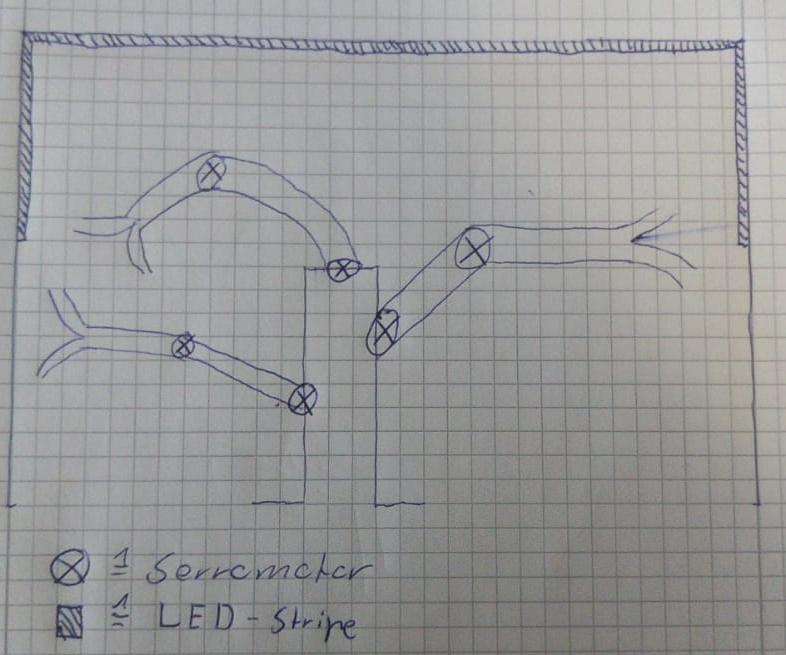
\includegraphics[
        width=0.5\linewidth,
    ]{imgs/tree_sketch.jpg}
    \caption{Erste Skizze des neuen Visualisierungskonzepts}
    \label{fig-tree-sketch}
    \end{center}
\end{figure}
\end{document}